
\section{Rigid Transformations}

Rigid transformations is a major topic in robotics. From perception, to kinematics and control, everywhere the concept of a rigid transformation appears. A rigid transformation defines the rotation and translation between two coordinate frames. How  both this translation, and specially this rotation, are represented (or parameterized) introduce fundamental concepts reviewed in the following paragraphes. 

Coordinate frames will be written as $\mathcal{F}^A,\ \mathcal{F}^B$, for frames~$A$ and~$B$. They could be positioned, for instance, at the pivot point of a platform and at the center point of a sensor.  

\subsection{Rotations}
There are several ways to represent a rotation. The most used ones are the following: rotation matrix, quaternion, Euler angles and axis angle. Each representation has benefits and drawbacks, depending on the application. For instance, for a sea ship which will never flip (hopefully), Euler angles could be a good option, but for an end effector tool expected to cover all orientations in 3D, quaternions or Rotation matrix could be better. 

\subsubsection{Rotation Matrix}
\paragraph{Definition} A rotation matrix~$\mathbf{R}$ is a squared, orthogonal matrix with $|\mathbf{R}|=1$. 

\paragraph{Interpretation} Columns of $\mathbf{R}$ can be interpreted as orthonormal vectors expressing a frame~$\mathcal{F}^B$ in terms of another frame~$\mathcal{F}^A$. In that case, such rotation matrix is expressed as~$\mathbf{R}^A_B$. Given two frames which are rotated, $\mathcal{F}^A$ and~$\mathcal{F}^B$, and given a vector~$\mathbf{v}^B$ expressed in terms of~$\mathcal{F}^B$, the following equation expresses the vector~$\mathbf{v}$ with its new coordinates in terms of~$\mathcal{F}^A$:
\begin{equation}
 \mathbf{v}^A = \mathbf{R}^A_B \mathbf{v}^B
\end{equation}
It fulfills also 
\begin{equation}
 \mathbf{v}^B = (\mathbf{R}^A_B)^{-1} \mathbf{v}^A = \mathbf{R}^B_A \mathbf{v}^A
\end{equation}

The number of parameters required for this parameterization is $n \times n$ in an $n$-dimension space. In 3D, for instance, 9 numbers are required. However, these 9 parameters have to fulfill certain conditions between them, so they are not free. These conditions are imposed by the definition of the rotation matrix itself: orthogonality and unit determinant.  

\paragraph{Chain of Rotations}
If a third frame~$\mathcal{F}^C$ is also rotated with respect to frame~$\mathcal{F}^B$, then the equation representing the chain of rotations, from a point expressed in terms of~$\mathcal{F}^C$ to the point expressed in terms of~$\mathcal{F}^A$, is: 
\begin{equation}
 \mathbf{v}^A = \mathbf{R}^A_B \mathbf{R}^B_C \mathbf{v}^C = \mathbf{R}^A_C \mathbf{v}^C
\end{equation}
Please be careful with the sequence of the matrix product representing the chain, since matrices are ordered from right to left, starting from the \textit{outer} rotation up to the \textit{inner} one. In the 3D case, computing~$\mathbf{R}^A_C$ requires 27 multiplications and 18 additions. 


\paragraph{Example in 2D}
In 2D, if frame~$\mathcal{F}^B$ is rotated by~$\alpha=30^o$ degrees with respect to frame~$\mathcal{F}^A$, the matrix representing this rotation is as follows: 
\begin{equation}
\mathbf{R}^A_B = 
\left[
\begin{array}{cc}
  \cos\alpha & -\sin\alpha\\
  \sin\alpha & \cos\alpha\\
\end{array}
\right] = 
\left[
\begin{array}{cc}
  \frac{\sqrt{3}}{2} & -\frac{1}{2}\\
  \frac{1}{2} & \frac{\sqrt{3}}{2}\\
\end{array}
\right] 
\end{equation}
Given $\mathbf{v}^B = [2\ 1]^T$ a vector (point) represented in terms of frame~$\mathcal{F}^B$, its coordinates in terms of frame~$\mathcal{F}^A$ are:
\begin{equation}
 \mathbf{v}^A = \mathbf{R}^A_B \mathbf{v}^B =
\left[
\begin{array}{cc}
  \frac{\sqrt{3}}{2} & -\frac{1}{2}\\
  \frac{1}{2} & \frac{\sqrt{3}}{2}\\
\end{array}
\right]
\left[
\begin{array}{c}
 2 \\
 1\\
\end{array}
\right] =
\left[
\begin{array}{c}
 1.232 \\
 1.866\\
\end{array}
\right]
\end{equation}
so $\mathbf{v}^A=[1.232\ 1.866]^T$ is the same point $\mathbf{v}$ but expressed in terms of frame~$\mathcal{F}^A$.


\subsubsection{Quaternions}
\paragraph{Definition} A quaternion[ref] is an extension of Complex numbers to 3D. As complex numbers can be represented as vectors in $\mathbb{R}^2$, quaternions can be represented as vectors in~$\mathbb{R}^4$, with one real part,~$a$, and three imaginary parts,~$b,c,d$: 
\begin{equation}
 \mathbf{q} = [q_r\ q_i\ q_j\ q_k]^T = 
    q_r\mathbf{1} + q_i\mathbf{i} + q_j\mathbf{j} + q_k\mathbf{k}=
    q_r + q_i\mathbf{i} + q_j\mathbf{j} + q_k\mathbf{k}, 
\end{equation}
so quaterions are defined over a base formed by vectors $\mathbf{1},\mathbf{i},\mathbf{j},\mathbf{k}$. Definition of this base is required to define the quaternion product. Vectors of this base fulfill:
\begin{itemize}
 \item $\mathbf{1}$ is the identity element $\rightarrow\ \mathbf{q}\mathbf{1} = \mathbf{q}$
 \item $\mathbf{i}\mathbf{i}=\mathbf{j}\mathbf{j}=\mathbf{k}\mathbf{k}=\mathbf{i}\mathbf{j}\mathbf{k}=-1$
 \item $\mathbf{i}\mathbf{j}=\mathbf{k};\ \mathbf{j}\mathbf{k}=\mathbf{i};\ \mathbf{k}\mathbf{i}=\mathbf{j};$
\end{itemize}

The \textbf{sum} of two quaternions, $\mathbf{q}^a$ and $\mathbf{q}^b$, is defined as the sum in $\mathbb{R}^4$:
\begin{equation}
 \mathbf{q} = \mathbf{q}^a + \mathbf{q}^b = [ (q^a_r+q^b_r)\ 
					      (q^a_i+q^b_i)\ 
					      (q^a_j+q^b_j)\
					      (q^a_k+q^b_k)\ ]^T
\end{equation}
and the \textbf{scalar product} of a quaternion is:
\begin{equation}
 u\mathbf{q} = [ uq_r\ uq_i\ uq_j\ uq_k]^T, \ \ u \in \mathbb{R}, 
\end{equation}
which also coincides with the scalar product in $\mathbb{R}^4$.

However, the \textbf{quaternion product} is quite more different than what we do with vectors in~$\mathbb{R}^4$. We use here the properties of the base $\{\mathbf{1,i,j,k}\}$ defined above, and the distributive law: 
\begin{equation}
 \mathbf{q} = \mathbf{q}^a \cdot \mathbf{q}^b =
 \left[
 \begin{array}{c}
    q^a_rq^b_r - q^a_iq^b_i - q^a_jq^b_j - q^a_kq^b_k\\
    q^a_rq^b_i + q^a_iq^b_r + q^a_jq^b_k - q^a_kq^b_j\\
    q^a_rq^b_j - q^a_iq^b_k + q^a_jq^b_r + q^a_kq^b_i\\
    q^a_rq^b_k + q^a_iq^b_j - q^a_jq^b_i + q^a_kq^b_r\\
 \end{array}
 \right]. 
%      m_aux = [p(1) -p(2) -p(3) -p(4); p(2:4) ( p(1)*eye(3,3) + skewMatrix(p(2:4)))];
%     q_out = m_aux*q;
\end{equation}

Finally, the \textbf{conjugate} of a quaternion is denoted as $\mathbf{q}^*$ and is computed as:
\begin{equation}
 \mathbf{q}^* = [q_r\ -q_i\ -q_j\ -q_k]^T
\end{equation}


\paragraph{Definition} \textbf{Unit quaternions} are those with unit norm,~$|\mathbf{q}|=1$. They are a way to represent rotations in 3D, usually not so intuitive, but with major practical benefits, specially in computer implementations. Let be a quaternion $\mathbf{q}^A_B$ a quaternion representing the rotation of frame~$\mathcal{F}^B$ with respect to frame~$\mathcal{F}^A$. Then, given a vector $\mathbf{v}^B$ expressed in terms of~$\mathcal{F}^B$, its components in terms of~$\mathcal{F}^A$ can be computed with the following equation: 
\begin{equation}
\left[
 \begin{array}{c}
 0\\
 v^A_x\\
 v^A_y\\
 v^A_z\\
 \end{array}
 \right] 
 =
 \mathbf{q}^A_B
 \cdot
 \left[
 \begin{array}{c}
 0\\
 v^B_x\\
 v^B_y\\
 v^B_z\\
 \end{array}
 \right]
 \cdot
 (\mathbf{q}^A_B)^*
\end{equation}
where the two product involved in the right side of the equation are quaternion products.  

\paragraph{Interpretation}
A good way to interpret 3D rotations represented by unit quaternions is to revisit how Complex numbers can represent 2D rotations. Let $\mathbf{c}=a+bi\ \in\mathbb{C}$ be a complex number with unit norm, $|\mathbf{c}|=1$. In that case, $\mathbf{c}$ is representing a point in the unit circle lying on the 2D plane, so it is also representing an angle $\alpha$ (FigureXX). This complex number can be written as:
\begin{equation}
 \mathbf{c} = \cos\alpha + \sin\alpha i
\end{equation}
Quaternions are an extension of this idea but exported to 3D, so they require three imaginary parts to fully represent a rotation, instead of a single imaginary part required in 2D:
\begin{equation}
 \mathbf{q} = \cos\frac{\alpha}{2} + u_x\sin\frac{\alpha}{2} \mathbf{i} + u_y\sin\frac{\alpha}{2} \mathbf{j} + u_z\sin\frac{\alpha}{2} \mathbf{k}
\end{equation}
where $\alpha$ is the angle over the rotation axis indicated by the vector $\mathbf{u}=[u_x\ u_y\ u_z]^T$. Therefore, if we rotate a vector over the Euclidean $X,Y$ or~$Z$ axes, we get a complex representations over each $x=0,y=0$ or~$z=0$ planes respectively. 

\paragraph{Chain of Rotations}
Unit quaternions behave very similarly to rotation matrix when chaining rotations. Lets involve three frames~$\mathcal{F}^A$,~$\mathcal{F}^B$ and~$\mathcal{F}^C$. $\mathbf{q}^A_B$ represents the rotation of frame~$B$ with respect to frame~$A$, and $\mathbf{q}^B_C$ represents the one of frame~$C$ with respect to~$B$. Then, $\mathbf{q}^A_C$, which is the rotation of frame~$C$ with respect to~$A$ is:
\begin{equation}
 \mathbf{q}^A_C = \mathbf{q}^A_B \cdot \mathbf{q}^B_C
\end{equation}
The operation required to compute~$\mathbf{q}^A_C$ performs 16 multiplications and 12 additions, so it is more computationally efficient than matrix chaining. This can be of relevance in real-time algorithms requiring massive computtaion of chains of rotations.

\paragraph{Conversion to Rotation Matrix}
Sometimes it can be useful to convert a quaternion to a rotation matrix. The formula below provides such conversion: 
\begin{equation}
\mathbf{R}(\mathbf{q}) = 2
\left[
\begin{array}{ccc}
\frac{1}{2} - q^2_2 - q^2_3 & q_1q_2-q_0q_3 & q_0q_2+q_1q_3 \\

q_0q_3+q_1q_2 & \frac{1}{2} - q^2_1 - q^2_3 &   q_2q_3-q_0q_1\\

q_1q_3-q_0q_2 & q_0q_1+q_2q_3 & \frac{1}{2} - q^2_1 - q^2_2
\end{array}
\right],
\end{equation}


\subsubsection{Axis Angle}
//TODO

\subsubsection{Euler Angles}
\paragraph{Definition}
Euler angles approach is an intuitive way to represent rotations, by expressing the three rotation angles applied to different orthogonal axis, in a given order. One of the most used conventions is the $Z-Y-X$ order, leading to three angles:
\begin{itemize}
  \item	Yaw, $\theta$, is the first angle, a rotation around the $Z$ axis of the reference frame, $\theta \in (-\pi, \pi]$.
  \item Pitch, $\phi$, is the second angle, a rotation around the current (once rotated) $Y$ axis, $\phi \in (-\pi/2, \pi/2]$.
  \item Roll, $\psi$, is the third angle, a rotation around the current (twice rotated) $X$ axis, $\psi \in (-\pi, \pi]$.
\end{itemize}
Figure~\ref{appF:fig:threeAngles} shows the order of the rotations of each euler angle to get the final orientation.
\begin{figure}[h]
\centering
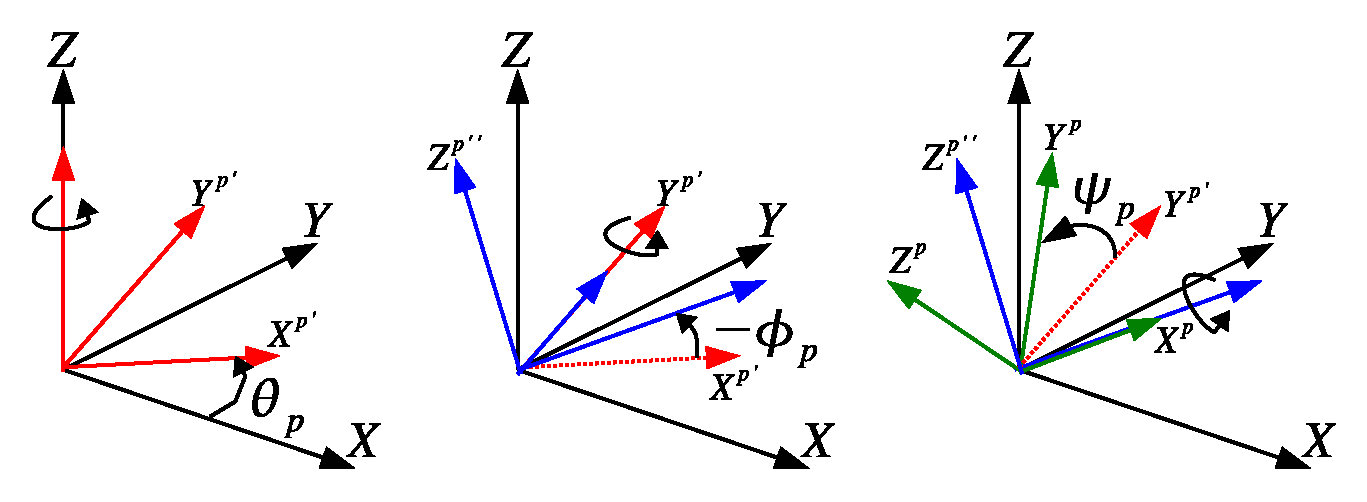
\includegraphics[height=4.2cm]{figures/threeAngles.eps}
\caption{Definition of the three euler angles yaw ($\theta$), pitch ($\phi$) and roll ($\psi$). Reference frame drawn in black. Intermediate frames drawn in red and blue. Final orientation frame shown in green. }
\label{appF:fig:threeAngles}
\end{figure}

\paragraph{Conversion to Rotation Matrix}
Since rotations are performed always around the current axis instead of around the fixed world axis, the whole rotation matrix is computed as:
\begin{equation}
 R(\theta,\phi,\psi) = R_{\theta,\phi,\psi} = R_z(\theta)R_y(\phi)R_x(\psi)
\end{equation}
where,
% //TODO: reedit matriz with [] style. And fit all in a single ``row''
%\begin{scriptsize}
\begin{equation}
\begin{split}
 & R_z(\theta)=
\begin{pmatrix}
 \cos\theta  & -\sin\theta & 0 \\
 \sin\theta & \cos\theta & 0 \\
 0          & 0         & 1 \\
\end{pmatrix}; \\
%\end{equation}
%\begin{equation}
%\label{appF:eq:R2} 
 & R_y(\phi)=
\begin{pmatrix}
 \cos\phi  & 0 & -\sin\phi \\
 0	    & 1	& 0 \\
 \sin\phi  & 0 & \cos\phi \\
\end{pmatrix};\\
%\end{equation}
%\begin{equation}
%\label{appF:eq:R3} 
 & R_x(\psi)=
\begin{pmatrix}
 1	       & 0 	& 0 \\
 0 & \cos\psi & -\sin\psi \\
 0 & \sin\psi & \cos\psi \\
\end{pmatrix};\\
\end{split}
\label{appF:eq:R123} 
\end{equation}
%\end{scriptsize}


\subsection{Adding translation}
Beyond rotations, a transformation may involve also a translation, which is the displacement between two frames, without taking into account their orientation. If two frames are translated, there is simply a vector to add between them: 
\begin{equation}
 \mathbf{v}^A = \mathbf{v}^B + \mathbf{p}^A_B
\end{equation}
where $\mathbf{p}^A_B$ is the vector expressing central point of frame~$B$ in terms of frame~$A$. 

When frame~$B$ is both rotated and translated with respect to frame~$A$, we apply first the rotation, and then the translation (see Figure~\ref{fig:rotation_translation}):
\begin{equation}
 \mathbf{v}^A = \mathbf{R}^A_B\mathbf{v}^B + \mathbf{p}^A_B
\end{equation}
\begin{figure}[bth!]
  \begin{center}
    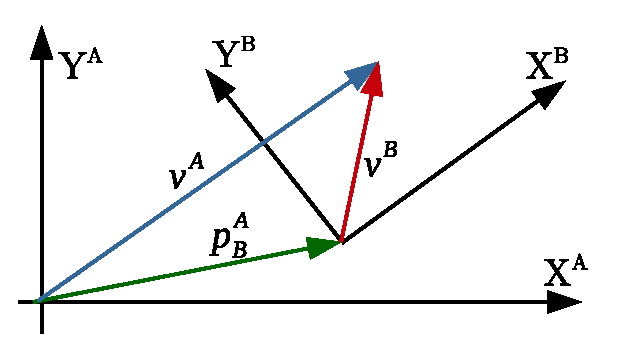
\includegraphics[width=1.0\columnwidth]{figures/rotation_translation.eps}
    \caption{Example of frame B, rotated and translated with respect to frame A.}
    \label{fig:rotation_translation}
  \end{center}
\end{figure}



\subsection{Homogeneous matrix}
Homogeneous matrix is a compact way to represent both rotation and translation in a single matrix, by adding an extra dimensionality to the rotation matrix.  
The homogeneous matrix representing the frame~$B$ in terms of the frame~$A$ (both rotation and translation) is defined as:
\begin{equation}
 \mathbf{T}^A_B = 
 \left[
 \begin{array}{cc}
  \mathbf{R}^A_B & \mathbf{p}^A_B \\
  0	& 	1 \\
 \end{array}
\right]
\end{equation}
Then, as it was described by pure rotation case in subsectionXX, it fulfills that:
\begin{equation}
\left[
 \begin{array}{c}
  \mathbf{v}^A \\
  1
 \end{array}
 \right]
 = \mathbf{T}^A_B 
 \left[
 \begin{array}{c}
  \mathbf{v}^B \\
  1
 \end{array}
 \right]; \ \
 \left[
 \begin{array}{c}
  \mathbf{v}^B \\
  1
 \end{array}
 \right]
  = (\mathbf{T}^A_B)^{-1} 
 \left[
 \begin{array}{c}
  \mathbf{v}^A \\
  1
 \end{array}
 \right].
\end{equation}
Homogeneous matrixes also allow chaining as rotations do:
\begin{equation}
 \left[
 \begin{array}{c}
  \mathbf{v}^A \\
  1
 \end{array}
 \right]
 = \mathbf{T}^A_B \mathbf{T}^B_C 
  \left[
 \begin{array}{c}
  \mathbf{v}^C \\
  1
 \end{array}
 \right]
 = \mathbf{T}^A_C \mathbf{v}^C
\end{equation}

\paragraph{Example}
As Figure~\ref{fig:world_vehicle_sensor_frames} draws, imagine we have a vehicle well localized at point $p^O=\left[p^O_x\ p^O_y\right]^T$ and oriented an angle~$\theta$ with respect to the origin of the trajectory. This vehicle has a sensor mounted at the known position~$m^B=[m^B_x\ m^B_y]$ and oriented an angle~$\beta$ with respect to the base frame of the vehicle. Finally this sensor has detected a point of interest at~$q^S=[q^S_x\ q^S_y]$. Which are the coordinates of the point of interest with respect to the base frame, and with respect to the origin of the trajectory ?
\begin{figure}[bth!]
  \begin{center}
    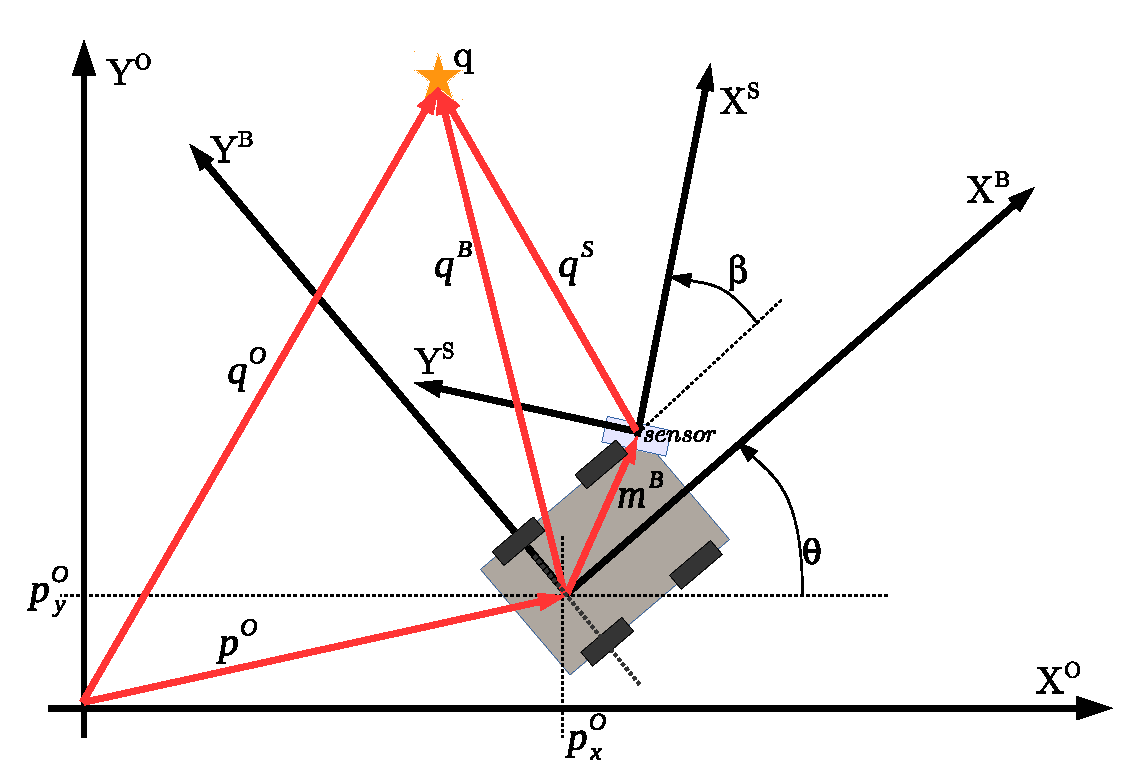
\includegraphics[width=1.0\columnwidth]{figures/world_vehicle_sensor_frames.eps}
    \caption{Trajectory, vehicle and sensor frames.}
    \label{fig:world_vehicle_sensor_frames}
  \end{center}
\end{figure}

The rotation matrixes involved are:
\begin{equation}
\mathbf{R}^O_B = 
\left[
 \begin{array}{cc}
    cos\theta   &  -sin\theta  \\
    sin\theta  & cos\theta \\
 \end{array}
 \right];\ \ 
\mathbf{R}^B_S = 
\left[
 \begin{array}{cc}
    cos\beta   &  -sin\beta  \\
    sin\beta  & cos\beta \\
 \end{array}
 \right];\ \ 
\end{equation}
and the homogeneous matrixes representing the transformations from the origin to the base, and from the base to the sensor, are respectively:
\begin{equation}
\mathbf{T}^O_B = 
\left[
 \begin{array}{cc}
    \mathbf{R}^O_B  &  p^0  \\
    \mathbf{0} & 1 \\
 \end{array}
 \right];\ \ 
\mathbf{T}^B_S = 
\left[
 \begin{array}{cc}
    \mathbf{R}^B_S  &  m^B  \\
    \mathbf{0} & 1 \\
 \end{array}
 \right];\ \ 
\end{equation}
So the point~$q$ with respect to the vehicle base frame and with respect to the origin of the trajectory is: 
\begin{equation}
\left[
\begin{array}{c}
    \mathbf{q}^B\\
    1 \\
 \end{array}
\right] = 
\mathbf{T}^B_S 
\left[
\begin{array}{c}
    \mathbf{q}_S\\
    1 \\
 \end{array}
\right];\ \ 
%%%%%%
\left[
\begin{array}{c}
    \mathbf{q}^O\\
    1 \\
 \end{array}
\right] = 
\mathbf{T}^O_B \mathbf{T}^B_S 
\left[
\begin{array}{c}
    \mathbf{q}_S\\
    1 \\
 \end{array}
\right];\ \ 
\end{equation}
  

\subsection{Choosing the right parameterization in 3D}
\begin{itemize}
 \item Nature and application of the vehicle/tool: ship, car, end-effector, camera, ...
 \item Differentation
 \item Dimensionality (Euler and quaternions only for 3D)
 \item ...
\end{itemize}
//TODO
